\documentclass[x11names, svgnames]{beamer}
\usepackage{listings}

\usetheme{sbi}

\title{RNA-Seq data analysis with Galaxy for clinical applications}
\author{Markus Wolfien \& Andrea Bagnacani}

\definecolor{Gray}{gray}{0.85}
\newcommand{\eg}{\textit{e}.\textit{g}.$\,\,$}

\begin{document}


%
% title
%
\frame[noframenumbering,plain]{\maketitle}



%
% outline
%
\newcommand{\one}{Who are we?}
\newcommand{\two}{Course outline}
\newcommand{\three}{RNA Sequencing (RNA-Seq)}
\newcommand{\four}{Next Generation Sequencing (NGS)}
\newcommand{\five}{Tools and materials}
\begin{frame}
  \frametitle{Outline}
  \begin{itemize}
    \itemsep1em
    \item \one
    \item \two
    \item \three
    \item \four
    \item \five
  \end{itemize}
\end{frame}



%
%
%
\begin{frame}
  \frametitle{\one}
  \begin{columns}[T]
    \begin{column}{0.5\textwidth}
      \begin{center}
        \vspace{-1em}
        
\includegraphics[scale=0.2]{images/logo_sbi}
      \end{center}
      \begin{center}
        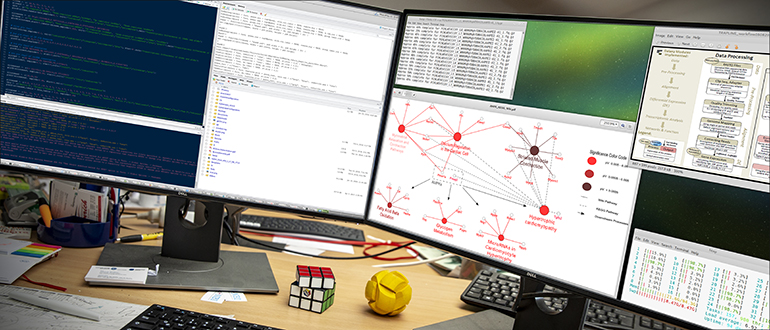
\includegraphics[scale=0.3]{images/markus_desk}
      \end{center}
    \end{column}
    \begin{column}{0.4\textwidth}
      \small{
      \begin{itemize}
        \vspace{-1em}
        \itemsep1em
        \item Data Management and standardisation
        \item Computational Modeling and Machine Learning
        \item Omics analysis and data integration
        \item Clinical trials
        \item Training courses
        \item eHealth
      \end{itemize}
      }
    \end{column}
  \end{columns}
\end{frame}
\begin{frame}
  \frametitle{\one}
  \begin{center}
    
\includegraphics[scale=0.08]{images/logo_denbi}
  \end{center}
  \begin{center}
    \footnotesize{\href{https://denbi.de}{\textcolor{gray}{https://denbi.de}}}
  \end{center}
  \begin{center}
    \vspace{2em}
    \textbf{de.STAIR}: Structured Analysis and Integration of RNA-Seq experiments (de.STAIR)
  \end{center}
  \begin{center}
    \small{Our aim is to provide and enable comprehensive analyses of RNA-Seq experiments as a service. To bring ease of use, reproducibility, and accessibility for the developed approaches and services, we provide dedicated workshops, training programs and screen casts for bioinformaticians and other life scientists.}
  \end{center}
\end{frame}
\begin{frame}
  \frametitle{\one}
  \begin{center}
    Who are you? :)
  \end{center}
\end{frame}



%
%
%
\begin{frame}
  \frametitle{\two}
  \begin{center}
    
\includegraphics[scale=0.1]{images/logo_github}
  \end{center}
  \begin{center}
    \footnotesize{\href{https://github.com/destairdenbi/trainings}{\textcolor{gray}{https://github.com/destairdenbi/trainings}}}
  \end{center}
\end{frame}



%
%
%
\begin{frame}
  \frametitle{\three}
  \begin{center}
  RNA-Seq is able to identify thousands of differentially expressed genes, tens of thousands of differentially expressed gene isoforms and can detect mutations and germline variations for hundreds to thousands of expressed genetic variants, as well as detecting chimeric gene fusions, transcript isoforms and splice variants.
  \end{center}
  \begin{center}
    \vspace{2em}
    \footnotesize{\href{https://doi.org/10.1038/nrg2484}{\textcolor{gray}{Wang, Nature 2009}}}
  \end{center}
\end{frame}
\begin{frame}
  \frametitle{\three}
  \begin{center}
    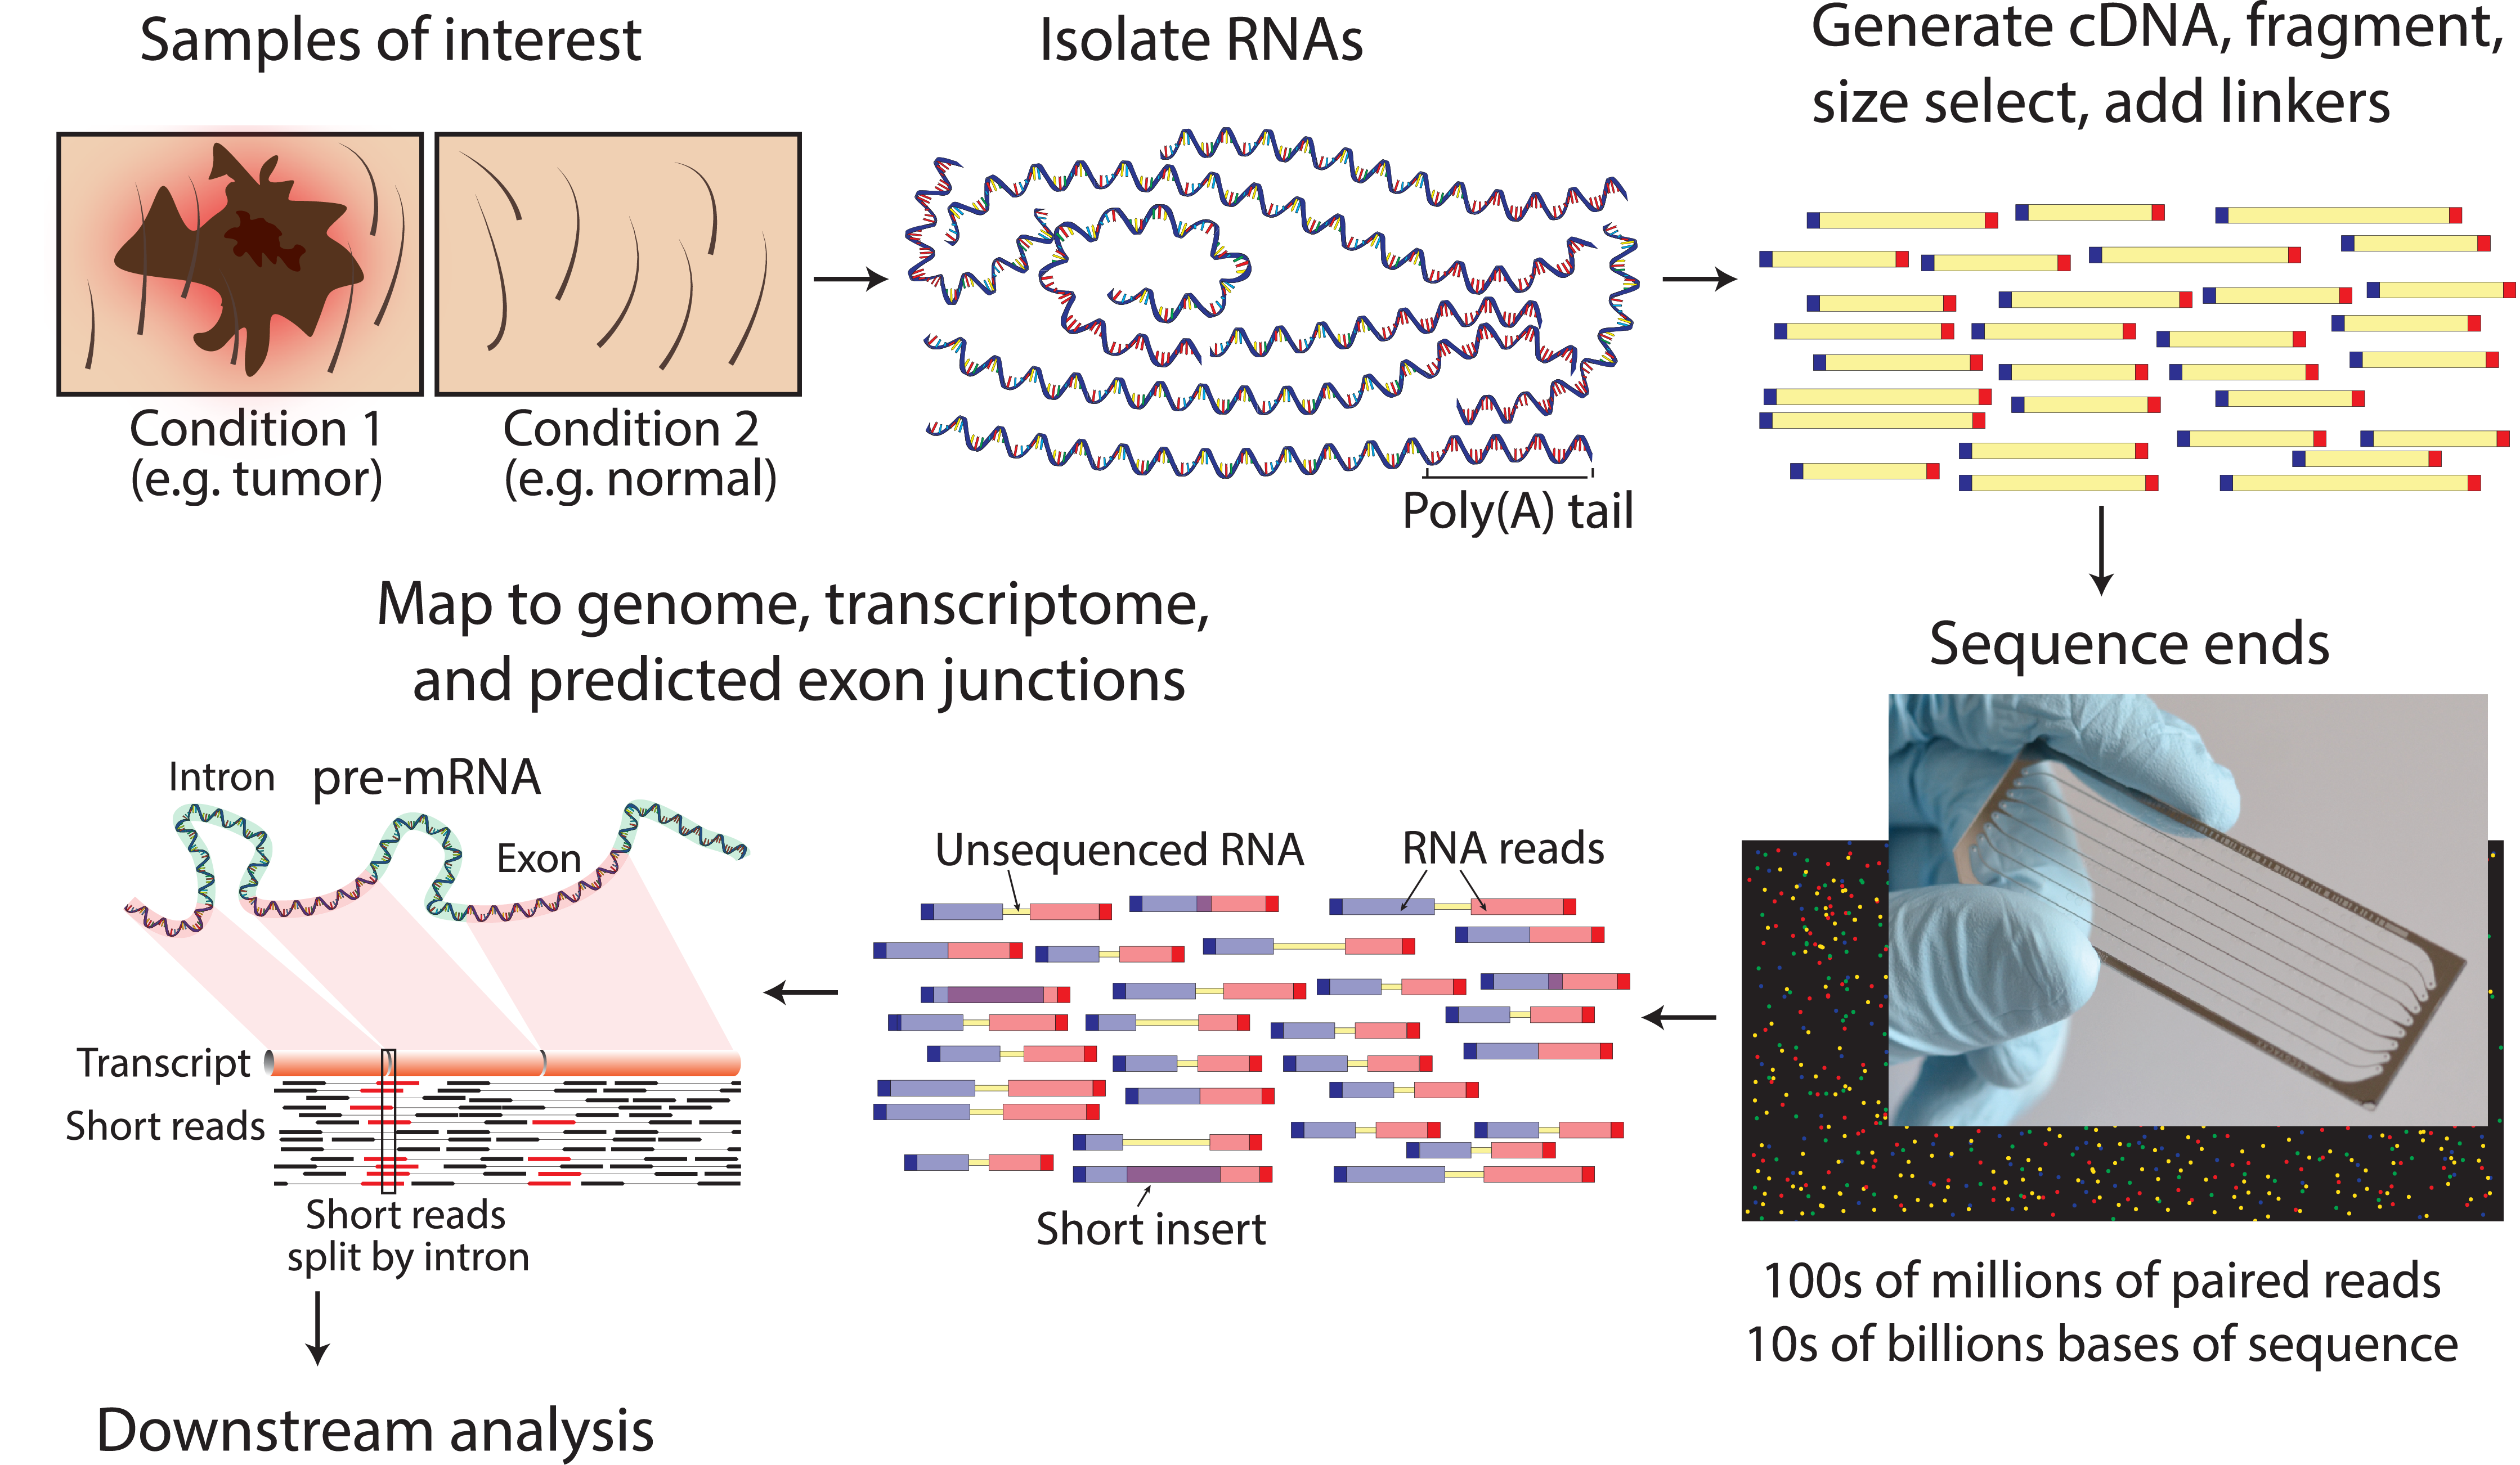
\includegraphics[scale=0.55]{images/griffith-plos}
  \end{center}
  \begin{center}
    \vspace{1.5em}
    \footnotesize{\href{https://doi.org/10.1371/journal.pcbi.1004393}{\textcolor{gray}{Griffith et al., PLOS 2015}}}
  \end{center}
\end{frame}



%
%
%
\begin{frame}
  \frametitle{\four}
  \begin{columns}[T]
    \begin{column}{0.5\textwidth}
      \begin{center}
        \vspace{-2em}
        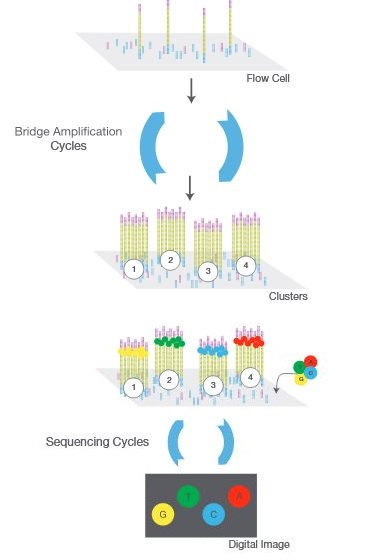
\includegraphics[scale=0.55]{images/illumina_sequencing}
      \end{center}
    \end{column}
    \begin{column}{0.5\textwidth}
      \begin{center}
        \vspace{-1em}
        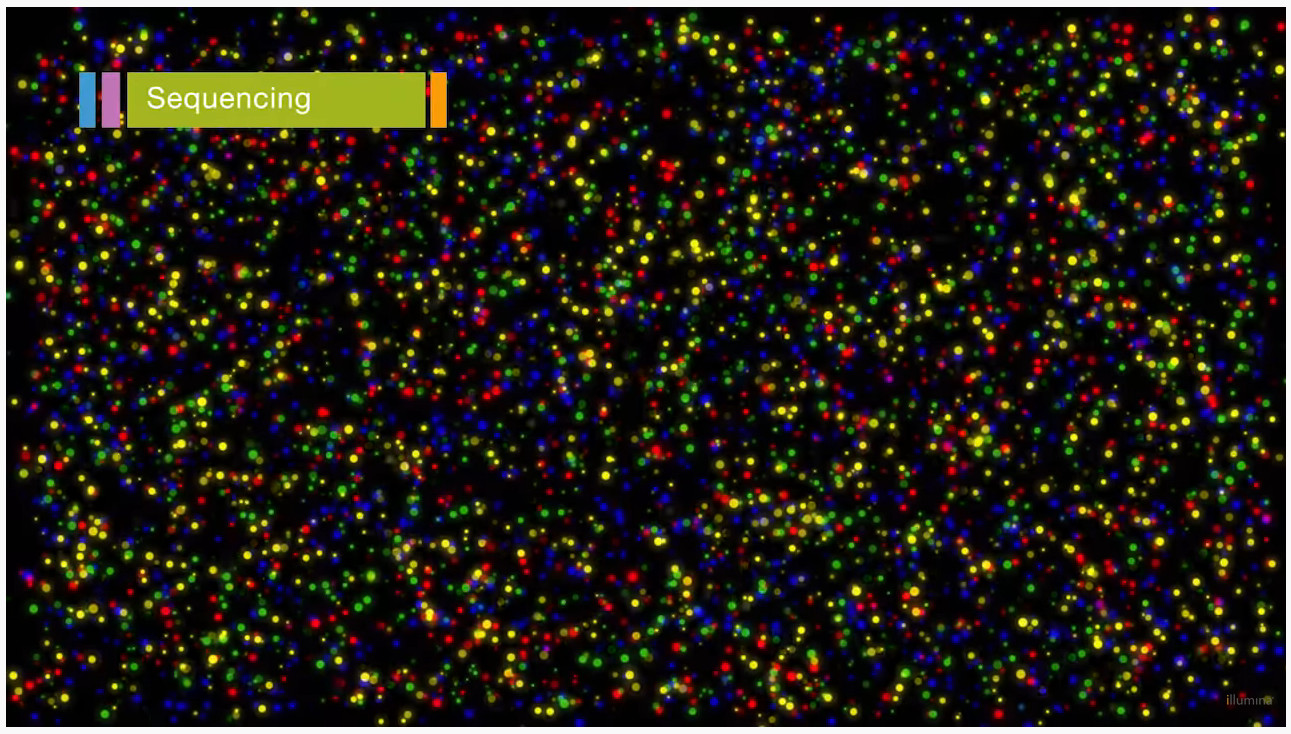
\includegraphics[scale=0.15]{images/illumina_video}
      \end{center}
      \begin{center}
        \tiny{\href{https://www.youtube.com/watch?v=fCd6B5HRaZ8}{\textcolor{gray}{https://www.youtube.com/watch?v=fCd6B5HRaZ8}}}
      \end{center}
      \vspace{4em}
      \footnotesize{
        \hfill\href{https://www.well.ox.ac.uk/ogc/sequencing-quality-monitoring-run/}{\textcolor{gray}{Oxford Genomics Centre, 2017}}
      }
      \vspace{6em}
      \footnotesize{
        \hfill\href{https://emea.illumina.com/content/dam/illumina-marketing/documents/products/other/ivf-reproductive-genetic-health-ngs-primer-1570-2015-012.pdf}{\textcolor{gray}{Illumina, 2015}}
      }
    \end{column}
  \end{columns}
\end{frame}
\begin{frame}
  \frametitle{\four}
  The decrease of sequencing costs is met with an increased effort in data processing $\implies$ Increased need of Bioinformatics expertise.
  \begin{center}
    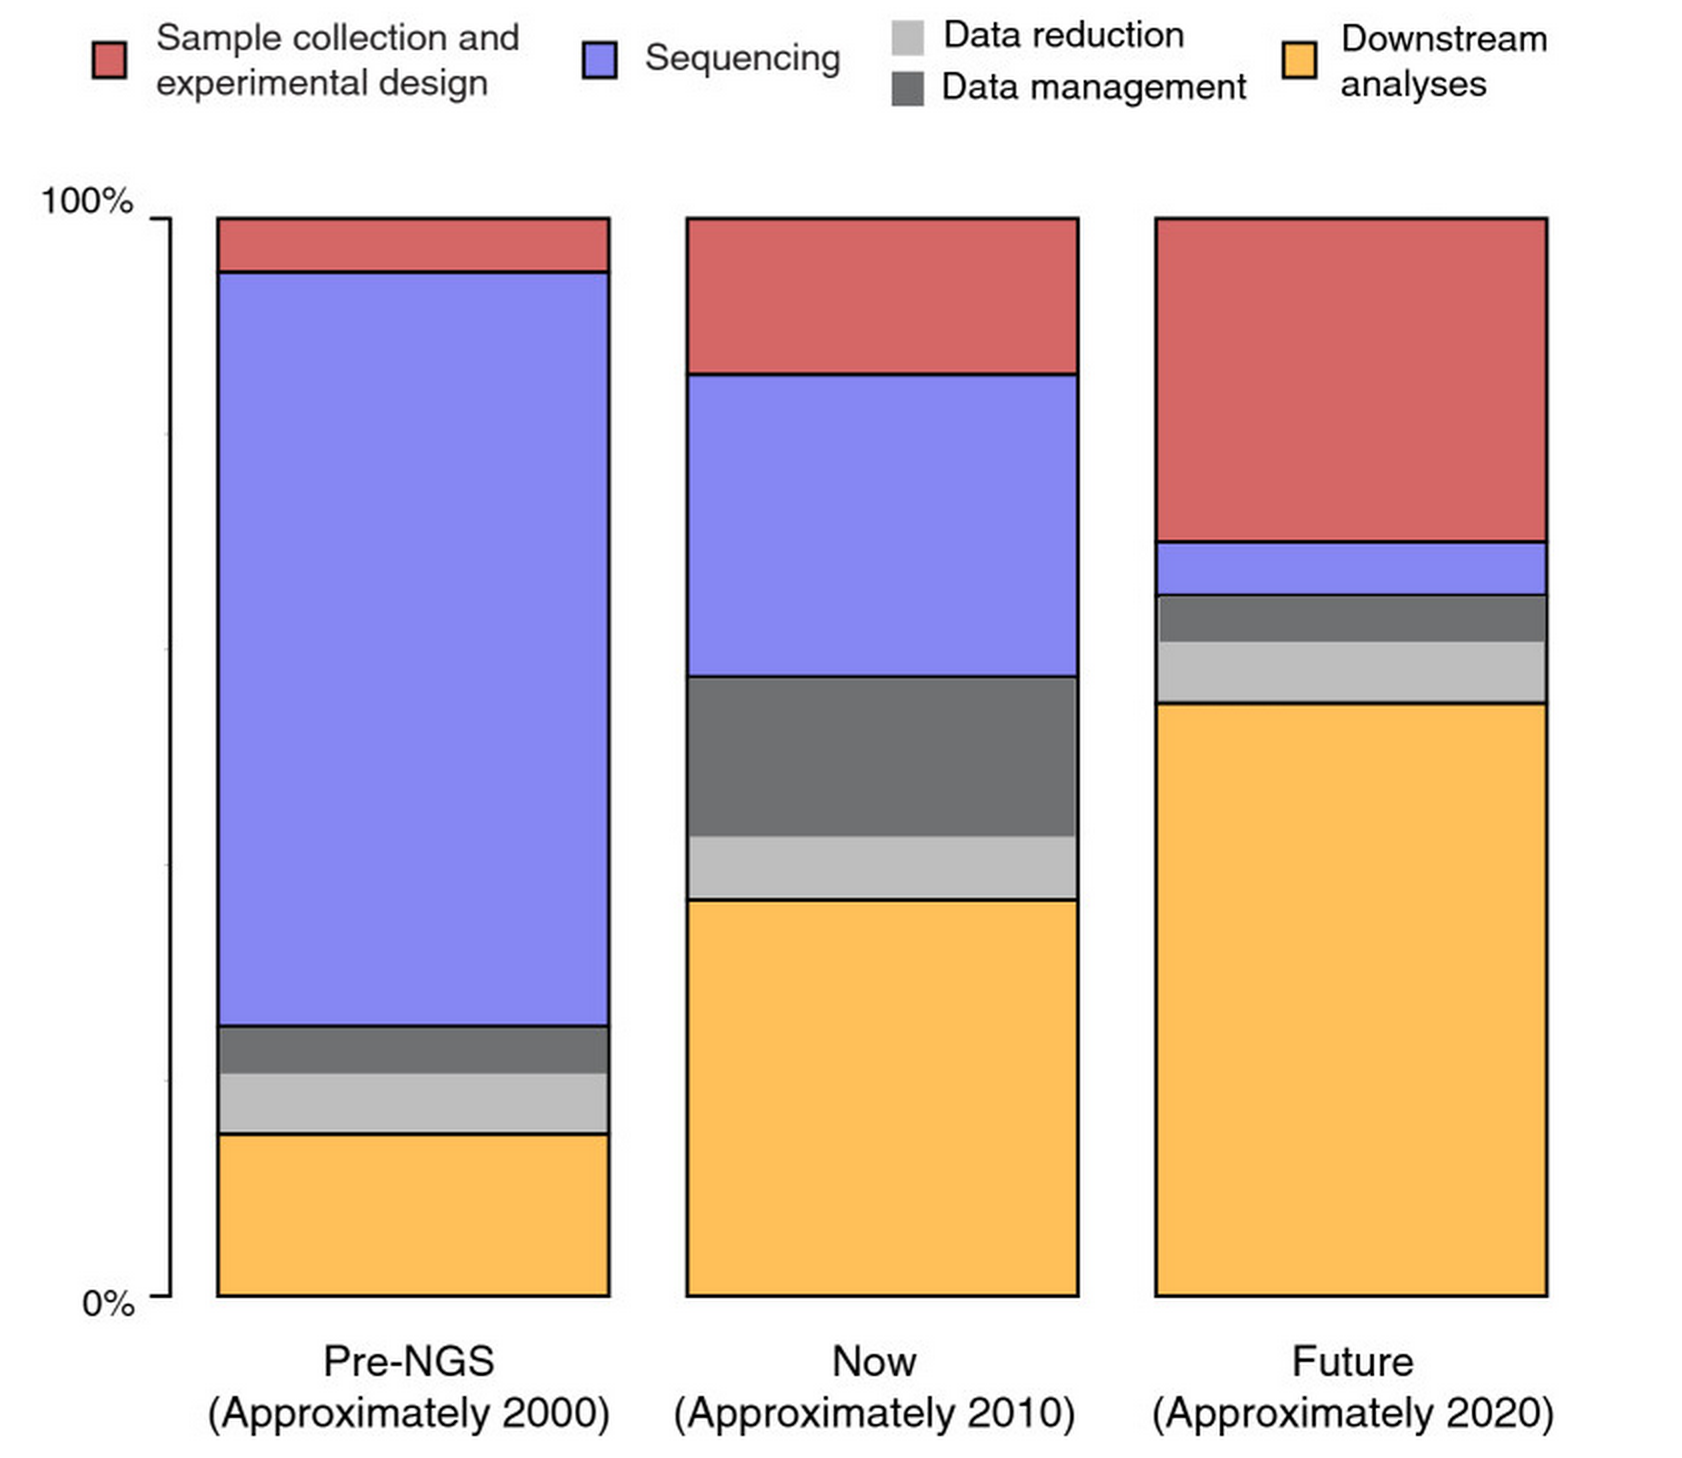
\includegraphics[scale=0.11]{images/sequencing_cost}
  \end{center}
  \begin{center}
    \vspace{-0.5em}
    \footnotesize{\href{https://doi.org/10.1186/gb-2011-12-8-125}{\textcolor{gray}{Sboner et al., Genome Biology 2011}}}
  \end{center}
\end{frame}



%
%
%
\begin{frame}
  \frametitle{\five}
  \begin{center}
    \vspace{-1em}
    
\includegraphics[scale=0.11]{images/logo_galaxy}
  \end{center}
  \begin{center}
    \footnotesize{\href{https://usegalaxy.eu}{\textcolor{gray}{https://usegalaxy.eu}}}
  \end{center}
  \begin{center}
    \vspace{2em}
    
\includegraphics[scale=0.11]{images/logo_gtn}
  \end{center}
  \begin{center}
    \footnotesize{\href{https://galaxyproject.github.io/training-material/}{\textcolor{gray}{https://galaxyproject.github.io/training-material/}}}
  \end{center}
\end{frame}

\end{document}
